\documentclass[a4paper,11pt]{article}
\usepackage{fullpage}
\usepackage{graphicx}
\usepackage{listings}
\usepackage{float}
\usepackage[section]{placeins}
\usepackage{setspace}
\usepackage{framed}

\title{DFN Statistics}
%\author{Name}
\begin{document}
\maketitle 
This file contains data regarding the results of the DFN generation process.

\begingroup
\def\addvspace#1{}
\tableofcontents
\endgroup

\section{General Info}
\lstinputlisting{report.txt}

\section{Mesh Info}
\lstinputlisting{finalmesh.txt}

\section{Time Profile}
\lstinputlisting{time_profile.txt}

\section{Discrete Fracture Network Visualization}
\begin{figure}[H]
  \centering
  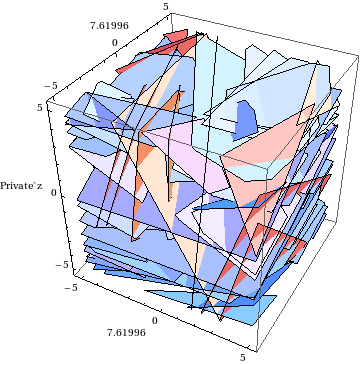
\includegraphics[width=300pt]{dfn.png}
  \caption[Discrete fracture network visualization]{Discrete Fracture Network visualization. Note: only the first 100 fractures are shown for DFNs with more than 150 fractures. In addition,the mesh and color are visual aids and do not represent the final mesh or family distribution.}
\end{figure}

\section{Family Distribution}
\begin{figure}[H]
  \centering
  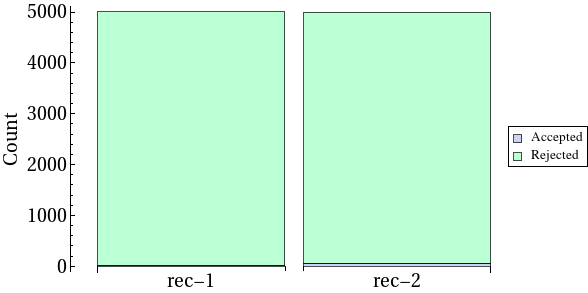
\includegraphics[width=300pt]{graphFamilyDist.png}
  \caption[Family distribution]{The final number of fractures for each defined family;as well as the number of attempts at arriving at the family distribution defined in the input file.}
\end{figure}

\section{Rejection Reasons}
\begin{figure}[H]
   \centering
    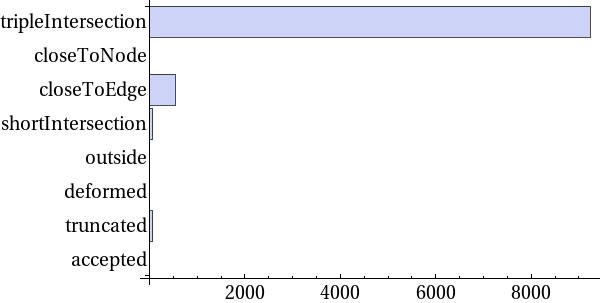
\includegraphics[width=300pt]{graphRejReasons.png} \caption[Rejection reasons]{Rejection reasons. Accepted: accepted and not truncated or deformed. Truncated: accepted and truncated (but not deformed) because part of the fracture was outside the domain. Deformed: accepted and truncated and deformed because of small features caused by truncation. Outside: rejected because only two or less vertices were inside the domain after truncation. ShortIntersection: rejected because an intersection shorter than h was created. CloseToEdge: rejected because an intersection was too close to an edge of the fractures. CloseToNode: rejected because an intersection was too close to a vertex of the fractures (this check is only performed for rectangular fractures). TripleIntersection: rejected because a triple intersection was created. }
\end{figure}

\lstinputlisting{rejReason.txt}

\section{Rejections per Fracture}
\begin{figure}[H]
  \centering
  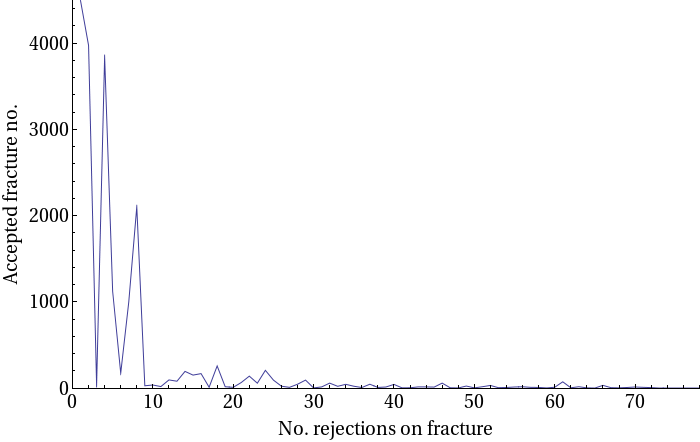
\includegraphics[width=300pt]{graphRejCaused.png}  \caption[Rejection per Fracture]{This figure illustrates the number of rejected fractures due to an invalid intersection with a specific fracture.}
\end{figure}

\section{Position Distribution}
\begin{figure}[H]
   \centering
    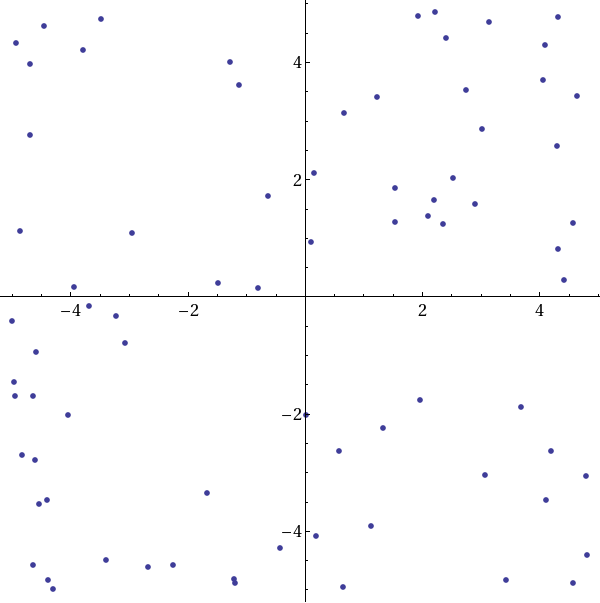
\includegraphics[width=300pt]{graphPositionDistribution.png} \caption{Position distribution.}
\end{figure}

\section{Normal Vectors}
\begin{figure}[H]
   \centering
    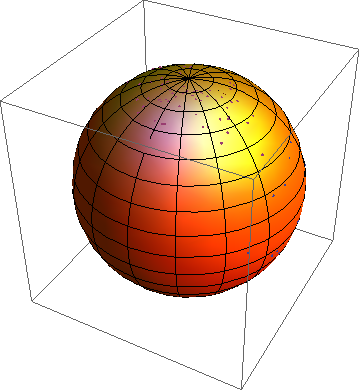
\includegraphics[width=300pt]{norm.png}
\caption[Normal vectors.]{Each point on the unit sphere represents the normal vector of an accepted fracture.Vectors from the same family have the same color points.}
\end{figure}


\section{Sizes of Connected Components}
\begin{figure}[H]
   \centering
   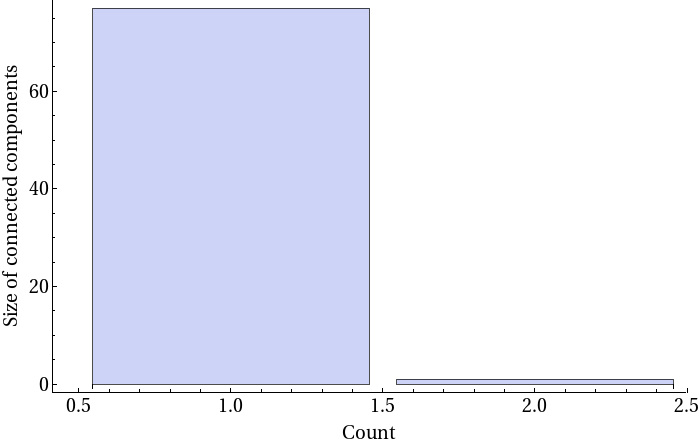
\includegraphics[width=300pt]{graphConnectedSize.png}
\caption[Sizes of connected components]{The number of fractures in each group of connected fractures (ordered from large to small). Ideally,the first group of connected fractures is much larger than the rest.}
\end{figure}

\section{Adjacency Matrix}
\begin{figure}[H]
  \centering
 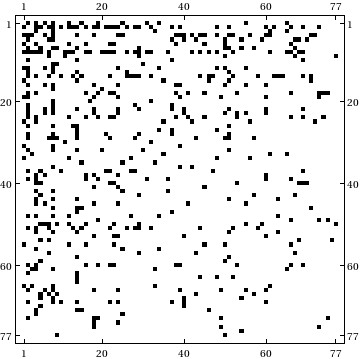
\includegraphics[width=300pt]{adj.png}
 \caption[Adjacency matrix]{Adjacency matrix. The axes are fracture numbers and a black square represents that the two corresponding fractures intersect. The matrix is symmetric. Note: when the matrix is large,it will appear denser then it actually is because of the resolution. }
\end{figure}

\section{Intersections Per Fracture}
\begin{figure}[H]
   \centering
    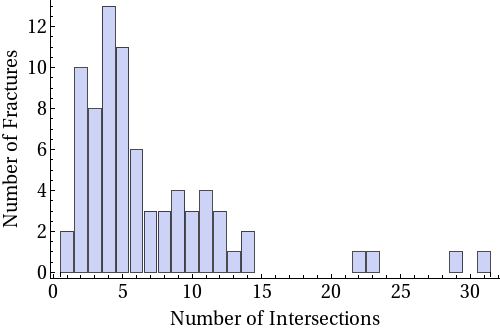
\includegraphics[width=300pt]{graphIntersectionNumber.png}
 \caption[Intersections Per Fracture]{The histogram of the number of intersections on each fracture.}
\end{figure}

\section{Boundary connections}
\begin{figure}[H]
   \centering
    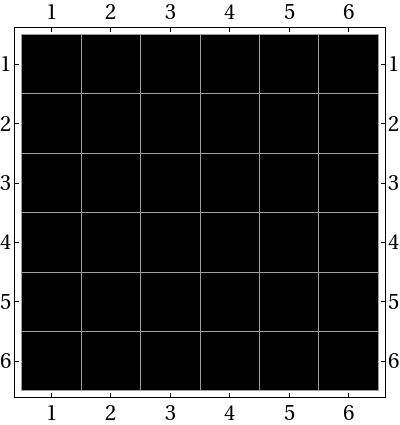
\includegraphics[width=300pt]{graphClusterInfo.png}
 \caption[Connectivity matrix]{Adjacency matrix for connectivity between domain boundaries: 1-top (Z+) , 2-bottom (Z-), 3-left (West) (X-), 4-front (South) (Y+), 5-right (East) (X+), 6-back (North) (Y-). The cell is colored black if there is a fracture cluster, which connects certain boundaries of the domain.}
\end{figure}

\section{Distribution of Generated Polygons' Lengths}
\begin{figure}[H]
  \centering
	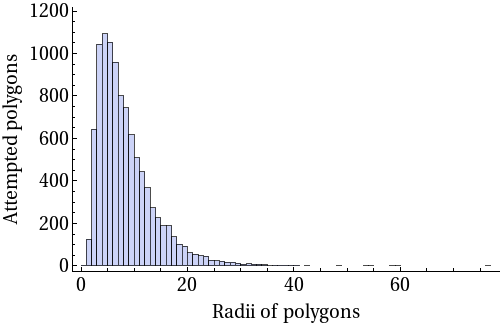
\includegraphics[width=300pt]{graphAttemptedDistribution.png}
  \caption{Distribution of generated polygon's length}
\end{figure}

%\section{Distribution of Generated Polygons' Lengths}
%\begin{figure}[H]
%\centering
%\includegraphics[width=300pt]{AttemptedDistribution_log.png}
%\caption[Distribution of generated polygon's length]{Distribution of generated polygon's length (in log-log scale).}
%\end{figure}

\section{Length Distribution of Fractures}
\begin{figure}[H]
   \centering
    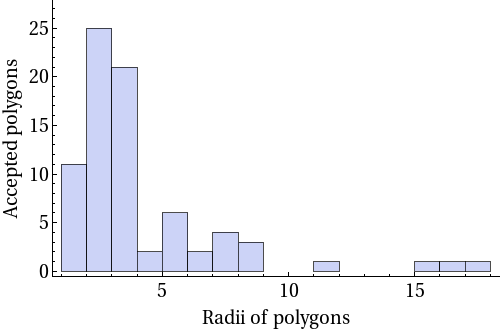
\includegraphics[width=300pt]{graphAcceptedDistribution.png}  \caption{Length Distribution of Fractures.}
\end{figure}

%\section{Length Distribution of Fractures}
%\begin{figure}[H]
%\centering
%\includegraphics[width=300pt]{AcceptedDistribution_log.png}
%\caption{Length Distribution of Fractures (in log-log scale).}
%\end{figure}

\newpage
\section{Mathematica Input File}
\lstinputlisting{mathInput.m}

\end{document}